% vim: set tw=0:
\documentclass{beamer}
\usepackage{graphicx}
\usepackage{hyperref}
\hypersetup{pdfborder={0 0 0 0}}

% Reasonable themes:
% Antibes Bergen Berkeley Berlin Frankfurt Goettingen Ilmenau Luebeck Malmoe
% Montpellier PaloAlto Rochester Singapore Szeged Warsaw bars boxes
% compatibility default lined plain shadow sidebar split tree
% And these ones include the author's name on every slide:
% Berkeley

% Declare themes.
\mode<presentation>
\usetheme{UWHEP}

% Personal macros.
\newcommand{\email}[1]{{\texttt #1}}
\newcommand{\newframe}[1]{\section{#1}
    \frametitle{\sc{#1}}}
\newcommand{\subframe}[1]{\subsection{#1}
    \frametitle{\sc{#1}}}
\newcommand{\supers}[1]{\ensuremath{^\textrm{#1}}}
\newcommand{\subs}[1]{\ensuremath{_\textrm{#1}}}
\newcommand{\ca}{\ensuremath{\sim}}
\renewcommand{\email}[1]{\href{mailto:#1}{\nolinkurl{#1}}}

% Author information.
\title{T2 Status}
\author[Maier, Mohapatra]{
    Will Maier \and Ajit Mohapatra\\
    {\tt wcmaier@hep.wisc.edu}\\
    {\tt ajit@hep.wisc.edu}}
\institute[Wisconsin]{University of Wisconsin - High Energy Physics}
\date{2009.11.10}
\logo{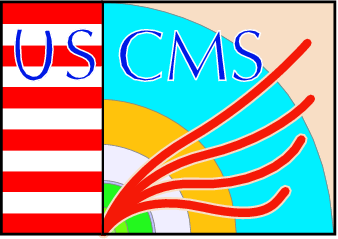
\includegraphics[height=0.6cm]{../../../Graphics/USCMS_logo.png}\hspace{.1cm}
\includegraphics[height=0.75cm]{../../../Graphics/UW_logo.png}}

\begin{document}

\begin{frame}
    \titlepage
\end{frame}

%\section{Overview}
%\begin{frame}
%    \tableofcontents
%\end{frame}

\section{Facilities}
\subsection{Software and Storage}
\begin{frame}
\frametitle{}

\begin{itemize}
	\item 2009.11.06: Lost filesystem on cmsgrid01 (OSG CE)
	\item Developing quotes to expand storage, replace PNFS server
	\item Lots of disk replacements
	\item Debugging failing/succeeding SAM tests on cmsgrid01
	\begin{itemize}
		\item SAM tests require {\tt \$HOME} environment variable
		\item In February, we removed {\tt \$HOME} from job environments for Nanohub
		\item This broke SAM tests, but {\tt sft-job} and {\tt prod} tests still showed 'Ok'
		\item Dashboard showed 'Ok' for other tests (from 2009.02.25)
		\item All should be fixed now; asked SAM folks to:
		\begin{itemize}
			\item display old results more clearly 
			\item not assume {\tt \$HOME} is set
			\item show an error if {\tt sft-job} or {\tt prod} tests fail
		\end{itemize}
	\end{itemize}
	\item Fixed incorrect mapping of JobRobot jobs to opportunistic resources
	\item 2009.10.27-28: Lost filesystem on PNFS server
	\begin{itemize}
		\item Another more-or-less simultaneous failure of three disks
		\item Rebuilt, but our old hotspare was running a rogue PnfsManager
		\item Brian saved the day
	\end{itemize}
\end{itemize}
\end{frame}

\subsection{Production and Monitoring}
\begin{frame}
\frametitle{}
\begin{itemize}
	\item JobRobot: OK
	\item SAM: OK
	\item RSV: OK
	\item PhEDEx:
	\begin{itemize}
		\item Both Prod and Debug instances running 3\_2\_9
		\item Bug in the FileRemove agent can make the agent very inefficient (reported yesterday in the FacOps HN)
		\item No major issues with the usual LT and Prod transfers
	\end{itemize}
	\item MC Production:
	\begin{itemize}
		\item Summer09 production continues: 750M events done between August and October
		\item 110M came last Wednesday; around 60M assigned to OSG (35M already done)
		\item Dorian is running production using one PA server at Wisconsin and using Omaha exclusively
		\item Will add UERJ and SPRACE to his PA and more US T3s to expand the OSG production coverage to more sites
	\end{itemize}
\end{itemize}
\end{frame}

\end{document}
